\documentclass{standalone}
\usepackage{tikz}
\usepackage{ctex,siunitx}
\setCJKmainfont{Noto Serif CJK SC}
\usepackage{tkz-euclide}
\usepackage{amsmath}
\usetikzlibrary{patterns, calc,3d}
\usetikzlibrary {decorations.pathmorphing,decorations.pathreplacing,decorations.shapes}
\begin{document}
\small
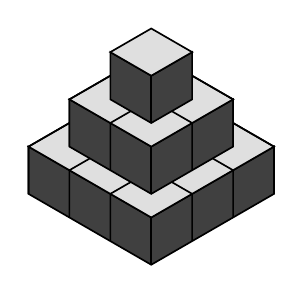
\begin{tikzpicture}[>=latex,scale=0.6]
  \draw[semithick,fill=darkgray](0,0)--(30:3)--++(0,1)--++(-150:3)--++(150:3)--++(0,-1)--cycle;
  \draw[semithick,fill=lightgray!50](0,1)--++(30:3)--++(150:3)--++(-150:3)--cycle;
  \foreach \x in {1,2,3}
  {
    \draw[semithick](30:\x)--++(0,1)--++(150:3);
    \draw[semithick](150:\x)--++(0,1)--++(30:3);
  }
  \draw[semithick,fill=darkgray](0,1.5)--++(30:2)--++(0,1)--++(-150:2)--++(150:2)--++(0,-1)--cycle;
  \draw[semithick,fill=lightgray!50](0,2.5)--++(30:2)--++(150:2)--++(-150:2)--cycle;
  \foreach \x in {1,2}
  {
    \draw[semithick]([yshift=1.5cm]30:\x)--++(0,1)--++(150:2);
    \draw[semithick]([yshift=1.5cm]150:\x)--++(0,1)--++(30:2);
  }
  \draw[semithick,fill=darkgray](0,3)--++(30:1)--++(0,1)--++(-150:1)--++(150:1)--++(0,-1)--cycle;
  \draw[semithick,fill=lightgray!50](0,4)--++(30:1)--++(150:1)--++(-150:1)--cycle;
  \draw[semithick](0,0)--(0,1)(0,1.5)--(0,2.5)(0,3)--(0,4);
\end{tikzpicture}
\end{document}